\documentclass[12pt]{article}
\usepackage{lmodern}
\usepackage{setspace}
\usepackage{amsfonts}
\usepackage{amsmath}
\usepackage{graphicx}
\setstretch{1.5}

%\DeclareMathSizes{12}{14}{10}{10}
\usepackage[margin=2.5cm]{geometry}    % How to set margins - optimized for 2.5cm      



%opening
\title{}
\author{}

\begin{document}

\maketitle



\section{Methodology}
\subsection{Overview}
Before delving into the specifics of employing reinforcement learning to the problem of automated trading, it will be informative to discuss the general theory and its underlying principles. 

Reinforcement learning aims to maximise a given reward signal by undertaking certain actions (in a restricted space). In this framework, an agent must take the state of the environment as input and take actions to alter the future state. A measurable goal related to the environment is also necessary in the problem formulation. Beyond this, each reinforcement learning problem contains four sub-elements: a \textit{policy}, a \textit{reward signal} and a \textit{value function}.\footnote{sutton book }

The policy defines the agent's actions in different environment states. The reward signal defines the goal and should be maximised over the course of the learning process. The value function maps the current state to a value so the agent can make optimal longer run decisions. It can be seen as the expected total future reward that can be obtained beginning from that state. Most of the challenges associated with the implementation of reinforcement learning derive from the estimation of the value function.

Formally, we construct a Markov Decision Process (MDP).
In an ideal situation, we would have access to the value function directly in tabular form when we have a tractable action and state space.

\begin{figure}
	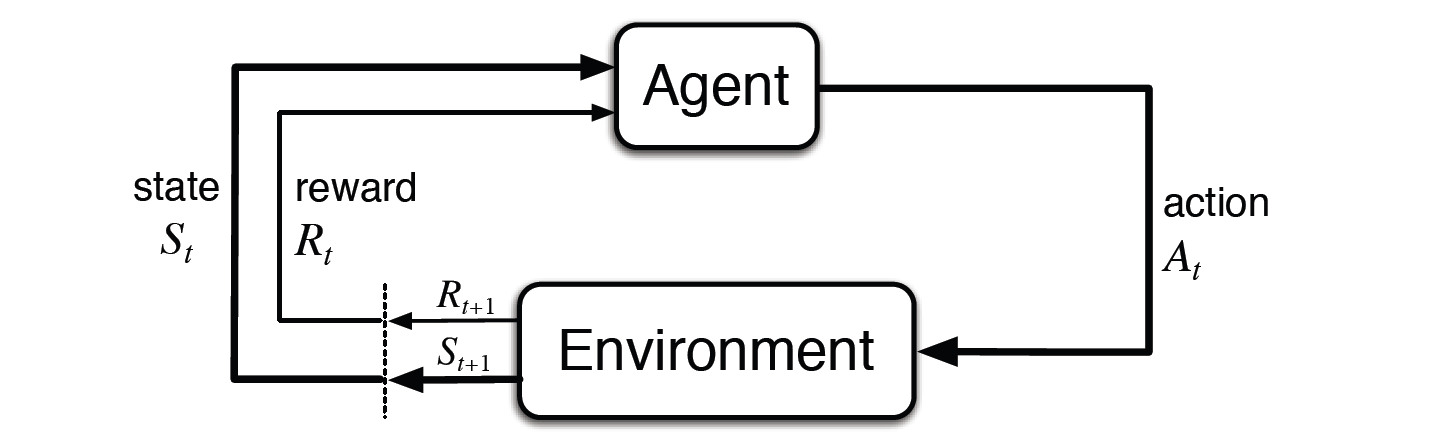
\includegraphics[width=\linewidth]{/Users/sammacintyre/Documents/StochRL/Loop.png}
	\caption{Agent and Environment Interaction}
	\label{fig:1}
\end{figure}

At a sequence of discrete time steps $t = 0,1,2,3...$, the agent interacts with the environment. At each step $t$, the agent receives state information $S _ { t } \in \mathcal{S}$ and performs an action $A _ { t } \in \mathcal { A } ( s )$. As a consequence of the action, the agent receives a reward $R _ { t + 1 } \in \mathcal { R } \subset \mathbb { R }$ and transitions to a new state $S _ { t + 1 }$.

In the context of a \textit{Markov} decision process, the future rewards ($R_{t}$) and states ($S_{t}$) only depend on the previous state and action. 

The general reinforcement learning paradigm involves find an optimal policy $\pi$ to maximise the expected discounted return. The discount factor is required to ensure that rewards in the distant future are less valuable than current rewards.

$$
G _ { t } \doteq R _ { t + 1 } + \gamma R _ { t + 2 } + \gamma ^ { 2 } R _ { t + 3 } + \cdots = \sum _ { k = 0 } ^ { \infty } \gamma ^ { k } R _ { t + k + 1 }
$$

Value and action-value functions allow the actions of the agent to be assessed under the implementation of a certain policy. The value function and action-value functions respectively are defined below:

$$
\begin{aligned}
v _ { \pi } ( s ) \doteq \mathbb { E } _ { \pi } \left[ G _ { t } | S _ { t } = s \right] = \mathbb { E } _ { \pi } \left[ \sum _ { k = 0 } ^ { \infty } \gamma ^ { k } R _ { t + k + 1 } | S _ { t } = s \right] , \text { for all } s \in \mathcal{S} \\
q _ { \pi } ( s , a ) \doteq \mathbb { E } _ { \pi } \left[ G _ { t } | S _ { t } = s , A _ { t } = a \right] = \mathbb { E } _ { \pi } \left[ \sum _ { k = 0 } ^ { \infty } \gamma ^ { k } R _ { t + k + 1 } | S _ { t } = s , A _ { t } = a \right]
\end{aligned}
$$ 

Ideally, the value function is decomposed into the following (known as the \textit{Bellman's Equation}):

$$
\begin{aligned} v _ { \pi } ( s ) & \doteq \mathbb { E } _ { \pi } \left[ G _ { t } | S _ { t } = s \right] \\ & = \mathbb { E } _ { \pi } \left[ R _ { t + 1 } + \gamma G _ { t + 1 } | S _ { t } = s \right] \\ & = \sum _ { a } \pi ( a | s ) \sum _ { s ^ { \prime } } \sum _ { r } p \left( s ^ { \prime } , r | s , a \right) \left[ r + \gamma \mathbb { E } _ { \pi } \left[ G _ { t + 1 } | S _ { t + 1 } = s ^ { \prime } \right] \right] \\ & = \sum _ { a } \pi ( a | s ) \sum _ { s ^ { \prime } , r } p \left( s ^ { \prime } , r | s , a \right) \left[ r + \gamma v _ { \pi } \left( s ^ { \prime } \right) \right] , \quad \text { for all } s \in S \end{aligned}
$$

Both expressions relate to a specific state and action taken at any time $t$.

A reinforcement learning problem principally involves pursuing the optimal policy $\pi$ which is is said to maximise the value and action-value functions:

$$
\begin{aligned}
v _ { * } ( s ) &\doteq \max _ { \pi } v _ { \pi } ( s )\\
q _ { * } ( s , a ) &\doteq \max _ { \pi } q _ { \pi } ( s , a )
\end{aligned}
$$

In the most simple cases where the value and action-value functions are specified, dynamic programming can be used to derive the optimal policy $\pi$.







In the algorithmic trading problem, the value function cannot be ascertained easily in this way. To deal with these situations and arbitrarily large state space, approximate solution methods must be used. This is known as a partially observable markov decision process as the state is only observed indirectly and cannot be fully known (we cannot know the trading behaviour of other agents for example) and we do not have access to the transition probabilities between states.

Q-Learning is a technique whereby the value functions are repeatedly estimated based on the rewards of our actions and assumes no prior model specification.


\subsection{Q-Learning} 

Q-learning attempts to estimate $q_{*}$ (optimal action-value function) without any regard for the policy followed.From a high level perspective, The Q-Learning algorithm proceeds by randomly initialising $q$, perform actions, measure reward and update $q$ accordingly. The final output after a training period should be a stable approximation of the $q_{*}$ table.

$$
\begin{array} { l } { \text { Algorithm parameters: step size } \alpha \in ( 0,1 ] , \text { small } \varepsilon > 0 } \\ { \text { Initialize } Q ( s , a ) , \text { for all } s \in \delta ^ { + } , a \in \mathcal { A } ( s ) , \text { arbitrarily except that } Q ( \text {terminal} , \cdot ) = 0 }  \\
\text{ Loop for each episode:} \\
\quad\text{ Initialize } S \\
\indent \text{ Loop for each step of episode:} \\
 \indent{ \text { Choose } A \text { from } S \text { using policy derived from } Q ( \text { e.g. } , \varepsilon \text { -greedy } ) } \\ \indent{ \text { Take action } A , \text { observe } R , S ^ { \prime } } \\ \indent { \hphantom{1}Q ( S , A ) \leftarrow Q ( S , A ) + \alpha \left[ R + \gamma \max _ { a } Q \left( S ^ { \prime } , a \right) - Q ( S , A ) \right] } \\ \indent{ \hphantom{1} S \leftarrow S ^ { \prime } }\\
\end{array}
$$ 


Notice the Bellman equation appearing in the update phase of the algorithm.

\subsubsection{Deep Q Learning}
An extension of this idea (which we aim to employ) is to use neural networks to approximate the Q-function.

A neural network is an appropriate tool for our use case due to the infinite nature of the state space. Estimating a table for each possible state would be excessive in regards to memory requirements.

To train the neural network on the state space, we must define a loss function. As The Bellman Equation defines the optimal result, we can use this to calculate our loss as follows:

$$
\begin{aligned}
\hat { Q } ( s , a ) &= R ( s , a ) + \gamma \max _ { a ^ { \prime } \in A } Q ( s , a ) \\
\text {Loss} &= \| Q - \hat { Q } \| _ { 2 }
\end{aligned}
$$

In general, a partition of the data is used to train the neural network and approximate the $q_{*}$ function, then this is used as our action-value function for deciding the optimal policy.

A neural network with 3 hidden layers was implemented in Tensorflow in our case.


\subsection{Problem formulation - Algorithmic Trading}
Now we must formualate the trading problem as a Markov Decision Process and define the states, actions and rewards.

\begin{itemize}
	\item State: $\mathcal{S} = \{prices,holdings,balance\} $ where $prices$ refers to the current prices of all the stocks in our portfolio, $holdings$ the quantity of each stock held and $balance$ as the total portfolio value
	\item Actions: $\mathcal{A} = \{buy,sell,hold\}$
	\item Rewards: $R_{t} \in \mathcal{R}$ can be defined as the change in the portfolio value due to an action $A_{t}$. Our Reward was defined as $R_{t} = balance_{t} - balance_{t-1}$
	\item Policy: $\pi$ which is governs the trading strategy at state $S$
	\item Action-value function: $q_{\pi}(s,a)$ as defined above. The expected reward we obtain by following policy $\pi$, choosing action $A$ while in state $S$. The action-value function is approximated by a neural network.
\end{itemize}

Initially we do not consider any transaction costs and only trade with a single stock (AAPL). Furthermore, a negative portfolio is not permissible ($balance_{t} \geq 0$ for all $t$).

In our primary model, the initial $balance_{0}$ is set to \$1000 and $price_{0}$ to the price of the stock at our chosen start time $t_{0}$ 




\section{Results}

Our neural network was set-up to learn from a 200 length rolling window (history) and as such, each state $S_{t}$ is a $200+2$ dimensional vector containing the history, the current budget ($balance_{t}$) and the current number of stocks held ($holdings_{t}$).

To ensure that the Q function was being learned in the correct way and trending towards an optimal policy, we train the neural network over multiple epochs. From the plot below, the final portfolio value achieved continues to increase, signalling convergence towards an optimal policy. The hyper-parameters were tweaked to derive maximum gain. (PLOT)

To evaluate the performance of the algorithm, we compared it to a standard \textit{Buy and Hold} strategy and to a randomised action strategy. The plots of the portfolio value over time below clearly demonstrate the superiority of Q-Learning, achieving a final portfolio profit of XXXX.

Despite the algorithm performing well, the \textit{Buy and Hold} strategy also performs similarly as AAPL is a strong stock with a stable upward trend.

To highlight the strength of Q-learning more effectively, we compared the algorithms behaviour on a more volatile stock, where \textit{Buy and Hold} should be less effective.

\subsection{Weaker stock comparison}

To illustrate how Q-Learning can out perform a \textit{Buy and Hold} strategy, we selected a stock with a less favourable trend over the past 10 years (WWL - Whiting Petroleum Corp.). Notably, the Q-learning algorithm clearly learns to buy low and sell high from its training, and out-performs \textit{Buy and Hold} dramatically.




\end{document}
